\documentclass[
  bibliography=totoc,     % Literatur im Inhaltsverzeichnis
  captions=tableheading,  % Tabellenüberschriften
  titlepage=firstiscover, % Titelseite ist Deckblatt
]{scrartcl}

% Paket float verbessern
\usepackage{scrhack}

% Warnung, falls nochmal kompiliert werden muss
\usepackage[aux]{rerunfilecheck}

% unverzichtbare Mathe-Befehle
\usepackage{amsmath}
% viele Mathe-Symbole
\usepackage{amssymb}
% Erweiterungen für amsmath
\usepackage{mathtools}

% Fonteinstellungen
\usepackage{fontspec}
% Latin Modern Fonts werden automatisch geladen
% Alternativ:
%\setromanfont{Libertinus Serif}
%\setsansfont{Libertinus Sans}
%\setmonofont{Libertinus Mono}
\recalctypearea % Wenn man andere Schriftarten gesetzt hat,
% sollte man das Seiten-Layout neu berechnen lassen

% deutsche Spracheinstellungen
\usepackage{polyglossia}
\setmainlanguage{german}


\usepackage[
  math-style=ISO,    % ┐
  bold-style=ISO,    % │
  sans-style=italic, % │ ISO-Standard folgen
  nabla=upright,     % │
  partial=upright,   % ┘
  warnings-off={           % ┐
    mathtools-colon,       % │ unnötige Warnungen ausschalten
    mathtools-overbracket, % │
},                       % ┘
]{unicode-math}

% traditionelle Fonts für Mathematik
\setmathfont{Latin Modern Math}
% Alternativ:
%\setmathfont{Libertinus Math}

\setmathfont{XITS Math}[range={scr, bfscr}]
\setmathfont{XITS Math}[range={cal, bfcal}, StylisticSet=1]

% Zahlen und Einheiten
\usepackage[
locale=DE,                   % deutsche Einstellungen
separate-uncertainty=true,   % immer Fehler mit \pm
per-mode=symbol-or-fraction, % / in inline math, fraction in display math
]{siunitx}

% chemische Formeln
\usepackage[
version=4,
math-greek=default, % ┐ mit unicode-math zusammenarbeiten
text-greek=default, % ┘
]{mhchem}

% richtige Anführungszeichen
\usepackage[autostyle]{csquotes}

% schöne Brüche im Text
\usepackage{xfrac}

% Standardplatzierung für Floats einstellen
\usepackage{float}
\floatplacement{figure}{htbp}
\floatplacement{table}{htbp}

% Floats innerhalb einer Section halten
\usepackage[
section, % Floats innerhalb der Section halten
below,   % unterhalb der Section aber auf der selben Seite ist ok
]{placeins}

% Seite drehen für breite Tabellen: landscape Umgebung
\usepackage{pdflscape}

% Captions schöner machen.
\usepackage[
  labelfont=bf,        % Tabelle x: Abbildung y: ist jetzt fett
  font=small,          % Schrift etwas kleiner als Dokument
  width=0.9\textwidth, % maximale Breite einer Caption schmaler
]{caption}
% subfigure, subtable, subref
\usepackage{subcaption}

% Grafiken können eingebunden werden
\usepackage{graphicx}
% größere Variation von Dateinamen möglich
\usepackage{grffile}

% schöne Tabellen
\usepackage{booktabs}

% Verbesserungen am Schriftbild
\usepackage{microtype}

% Literaturverzeichnis
\usepackage[style=alphabetic,]{biblatex}
% Quellendatenbank
\addbibresource{lit.bib}
\addbibresource{programme.bib}

% Hyperlinks im Dokument
\usepackage[
  unicode,        % Unicode in PDF-Attributen erlauben
  pdfusetitle,    % Titel, Autoren und Datum als PDF-Attribute
  pdfcreator={},  % ┐ PDF-Attribute säubern
  pdfproducer={}, % ┘
]{hyperref}
% erweiterte Bookmarks im PDF
\usepackage{bookmark}

% Trennung von Wörtern mit Strichen
\usepackage[shortcuts]{extdash}

\title{US1: Grundlagen der Ultraschalltechnik}
\author{
  Simon Schulte
  \texorpdfstring{
    \\
    \href{mailto:simon.schulte@udo.edu}{simon.schulte@udo.edu}
  }{}
  \texorpdfstring{\and}{, }
  Tim Sedlaczek
  \texorpdfstring{
    \\
    \href{mailto:tim.sedlaczek@udo.edu}{tim.sedlaczek@udo.edu}
  }{}
}
\publishers{TU Dortmund – Fakultät Physik}

\date{Durchführung: 04.07.2017\\
      Abgabe: 11.07.2017}


\begin{document}

\maketitle
\thispagestyle{empty}
\tableofcontents
\newpage
\setcounter{page}{1}
\section{Zielsetzung}
\label{sec:zielsetzung}
Bei diesem Versuch wird die Schallgeschwindigkeit und Dämpfung von Ultraschall
in Acryl untersucht. Anschließend werden an einem Augenmodell Distanzen gemessen.
\section{Theorie}
\label{sec:theorie}
Als Ultraschall werden Schallwellen mit Frequenzen zwischen $\SI{20}{\kilo\hertz}$
und $\SI{1}{\giga\hertz}$ bezeichnet.
Ihre Intensität nimmt bei der Ausbreitung nach
\begin{equation}
  I \left( x \right) = I_0 \cdot e^{-\alpha x}
  \label{eqn:dämpfung}
\end{equation}
ab. $\alpha$ ist dabei der Absorptionskoeffizient.\\
\\
\noindent
Für die Erzeugung von Ultraschall wird der piezo-elektrische Effekt verwendet.
Hierbei wird ein geeigneter Kristall elekrisch zu Schwingungen angeregt.
Die Resonanz des Kristalls kann dabei auch zur Messung von Ultraschall verwendet
werden.\\
\\
\noindent
Bei Messungen mit Ultraschall gibt es allgemein zwei verschiedene Methoden.
Das Durchschallungs-Verfahren und das Impuls-Echo-Verfahren.\\
Bei dem Durchschallungs-Verfahren werden zwei Ultraschallsonden verwendet.
Die erste agiert als Sender und die zweite als Empfänger. Zischen den
Sonden wird die Probe platziert. Durch Messung der Zeitpunkte der Impulse
lässt sich so bei bekannter Schallgeschwindigkeit die Länge bzw. bei bekannter
Länge die Schallgeschwindigkeit der Probe bestimmen.\\
Bei dem Impuls-Echo-Verfahren wird nur eine Sonde verwendet. Diese agiert
als Sender und Empfänger. Durch Laufzeitmessungen lassen sich auch hier
Länge und Schallgeschwindigkeit der Probe bestimmen. Im Gegensatz zum
Durchschallungs-Verfahren kann hierbei auch die Position von potenziellen
Fehlstellen bestimmt werden.
Da der Schall bei dieser Methode immer den doppelten Weg zurücklegt ergibt sich
für die Strecke
\begin{equation}
  s = \frac{1}{2}\,c\,t
  \label{eqn:strecke}
\end{equation}
\clearpage
\section{Durchführung}
\label{sec:durchführung}
\subsection{Versuchsaufbau}
\label{sec:aufbau}
Der Aufbau besteht aus einem Ultraschallgenerator, an dem zwei Sonden
angeschlossen sind. An einem Drehschalter ist auswählbar, welche Sonden Jeweils
Sender und Empfänger sein sollen. Es stehen mehrere Acrylzylinder und Platten
mit unterschiedlichen Längen bzw. Dicken zur Verfügung. Für das
Durchschallungs-Verfahren liegt ein Keil vor, welcher dafür sorgt, dass
die Zylinder nicht wegrollen. Die Daten der Sonden werden an einem Computer
angezeigt. Daran lassen sich dann die Laufzeiten und Signalamplituden bestimmen.
Für den letzten Versuchsteil wird ein Augenmodell verwendet, wie es in Abbildung
\ref{fig:auge} dargestellt ist.
\begin{figure}[H]
  \centering
  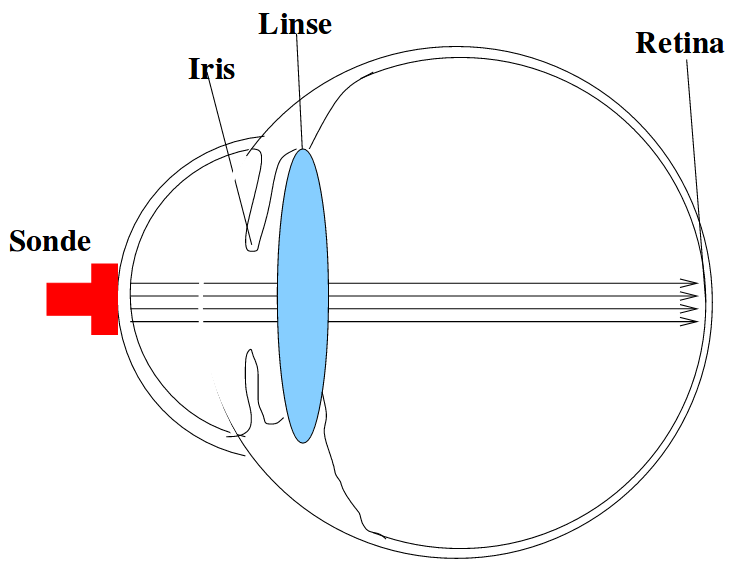
\includegraphics[width=0.5\textwidth]{Augenmodell.png}
  \caption{Schematische Darstellung des Augenmodells. \cite{anleitung}}
  \label{fig:auge}
\end{figure}
\noindent
Für die Zylinder und Platten wurden vorab folgende Längen gemessen:
\begin{table}
  \centering
  \caption{Zylinderlängen.}
  \label{tab:größen}
  \sisetup{table-format=2.3}
  \begin{tabular}{S[table-format=1.0] S}
    \toprule
    {Zylinder/Platte Nr.} & {Länge/Dicke in \si{\centi\meter}} \\
    \midrule
    1 &  3.115 \\
    2 &  4.045 \\
    3 &  6.160 \\
    4 &  7.086 \\
    5 &  8.045 \\
    6 & 10.240 \\
    7 & 12.055 \\
    a &  0.610 \\
    b &  1.195 \\
    \bottomrule
  \end{tabular}
\end{table}\\
\noindent
Zylinder Nr.4 wird dabei aus einem Zylinder der Länge $\SI{3}{\centi\meter}$
und einem der Länge $\SI{4}{\centi\meter}$ zusammengesetzt und die Buchstaben
stehen für die Acrylplatten.
\clearpage
\subsection{Versuchsablauf}
\label{sec:ablauf}
Zuerst wird mit dem Impuls-Echo-Verfahren die Laufzeit und die Amplitude der
Impulse in den verschiedenen Zylindern gemessen. Damit lässt sich die
Schallgeschwindigkeit in Acryl und der entsprechende Absorptionskoeffizient
bestimmen.
Anschließend werden alle Zylinder außer Nr.4 mit dem Durchschallungs-Verfahren
erneut vermessen. Hierbei wird nur die Laufzeit notiert.\\
\\
\noindent
Nun werden die beiden Acrylplatten aufeinander und Zylinder Nr.2 auf den beiden
Platten platziert. Von oben wird dann per Impuls-Echo-Verfahren ein Cepstrum
aufgenommen. Dieses zeigt ein Spektrum aus Laufzeiten, die durch mehrfache
Reflexion entstehen. Anhand dieser kann die Dicke der Platten bestimmt werden.\\
\\
\noindent
Zuletzt werden an einem Augenmodell per Impuls-Echo-Verfahren die Abstände
zwischen Iris, Linse und Retina bestimmt.
\clearpage

\section{Auswertung}
\subsection{Bestimmung der Schallgeschwindigkeit in Acryl}
Die aus der Messung nach dem Impuls-Echo-Verfahren gewonnenen Messwerte finden sich
in Tabelle \ref{tab:1}, die aus dem Durchschallungsverfahren in Tabelle \ref{tab:2}.
  \begin{table}
    \centering
    \begin{tabular}{c c c c}
      \toprule
      $l$/\si{\milli\metre} & $U$/\si{\volt} & $t$/\si{\micro\second} & TGC/\si{\decibel} \\
      \midrule
      40.45  & 0.60 & 29.6 & 0  \\
      80.45  & 0.19 & 58.8 & 10 \\
      120.55 & 0.07 & 88.2 & 20 \\
      102.40 & 0.06 & 75.6 & 20 \\
      31.15  & 0.62 & 23.0 & 0  \\
      61.60  & 0.08 & 45.5 & 0  \\
      70.85  & 0.05 & 53.2 & 0  \\
      \bottomrule
    \end{tabular}
    \caption{Messwerte der Messung per Impuls-Echo-Verfahren.}
    \label{tab:1}
  \end{table}
  \begin{table}
    \centering
    \begin{tabular}{c c c c}
      \toprule
      $l$/\si{\milli\metre} & $U$/\si{\volt} & $t$/\si{\micro\second} & TGC/\si{\decibel} \\
      \midrule
      31.15  & 0.729 & 23.2 & 0 \\
      40.45  & 0.759 & 29.5 & 0 \\
      61.60  & 0.271 & 46.6 & 0 \\
      80.45  & 0.154 & 39.1 & 0 \\
      102.40 & 0.271 & 38.5 & 0 \\
      120.55 & 0.329 & 45.0 & 0 \\
      \bottomrule
    \end{tabular}
    \caption{Messwerte der Messung per Durchschallungsverfahren.}
    \label{tab:2}
\end{table}
Hierbei bezeichnet $l$ jeweils die Höhe der Zylinder, $U$ die Spannungsamplitude des
gemessenen Peaks, $t$ den zeitlichen Abstand zwischen senden des Schallimpulses
und empfangen des Signals und TGC gibt den verwendeten Verstärkungsfaktor für
den Amplitudenwert an.
Die Bestimmung der Schallgeschwindigkeiten geschieht nun durch lineare Regression.
Zu beachten ist, dass sich die Laufzeiten bei der Messung per Impuls-Echo-Verfahren
verfahrensbedingt auf die doppelte Länge beziehen. Es werden daher in den Rechnungen die halben gemessenen
Laufzeiten betrachtet.
Dies ist notwendig, da innerhalb des Sondenmaterials eine gewisse Strecke zurückgelegt werden
muss, die ansonsten als systematischer Fehler in die Rechnung eingehen würden.
Die Regression der Länge-Laufzeit Wertepaare errechnet sich mit
\begin{equation}
  t(l) = l \cdot \frac{1}{c} + t_0 .
\end{equation}
Dabei ist $c$ die Schallgeschwindigkeit im Zylinder und $t_0$ die Laufzeit innerhalb der
Sonde. Das liefert für das Impuls-Echo-Verfahren:
\begin{align*}
  c &= \SI[per-mode=reciprocal]{2713(24)}{\metre\per\second}\\
  t_0 &= \SI{1.0(1)}{\micro\second}
\end{align*}
und für das Durchschallungsverfahren:
\begin{align*}
  c &= \SI[per-mode=reciprocal]{2731(27)}{\metre\per\second}\\
  t_0 &= \SI{1.6(2)}{\micro\second}
\end{align*}
Messwerte und Regression sind in Abbildung \ref{abb:1} für das Impuls-Echo-Verfahren,
sowie in Abbildung \ref{abb:2} für das Durchschallverfahren dargestellt.
\begin{figure}
  \centering
    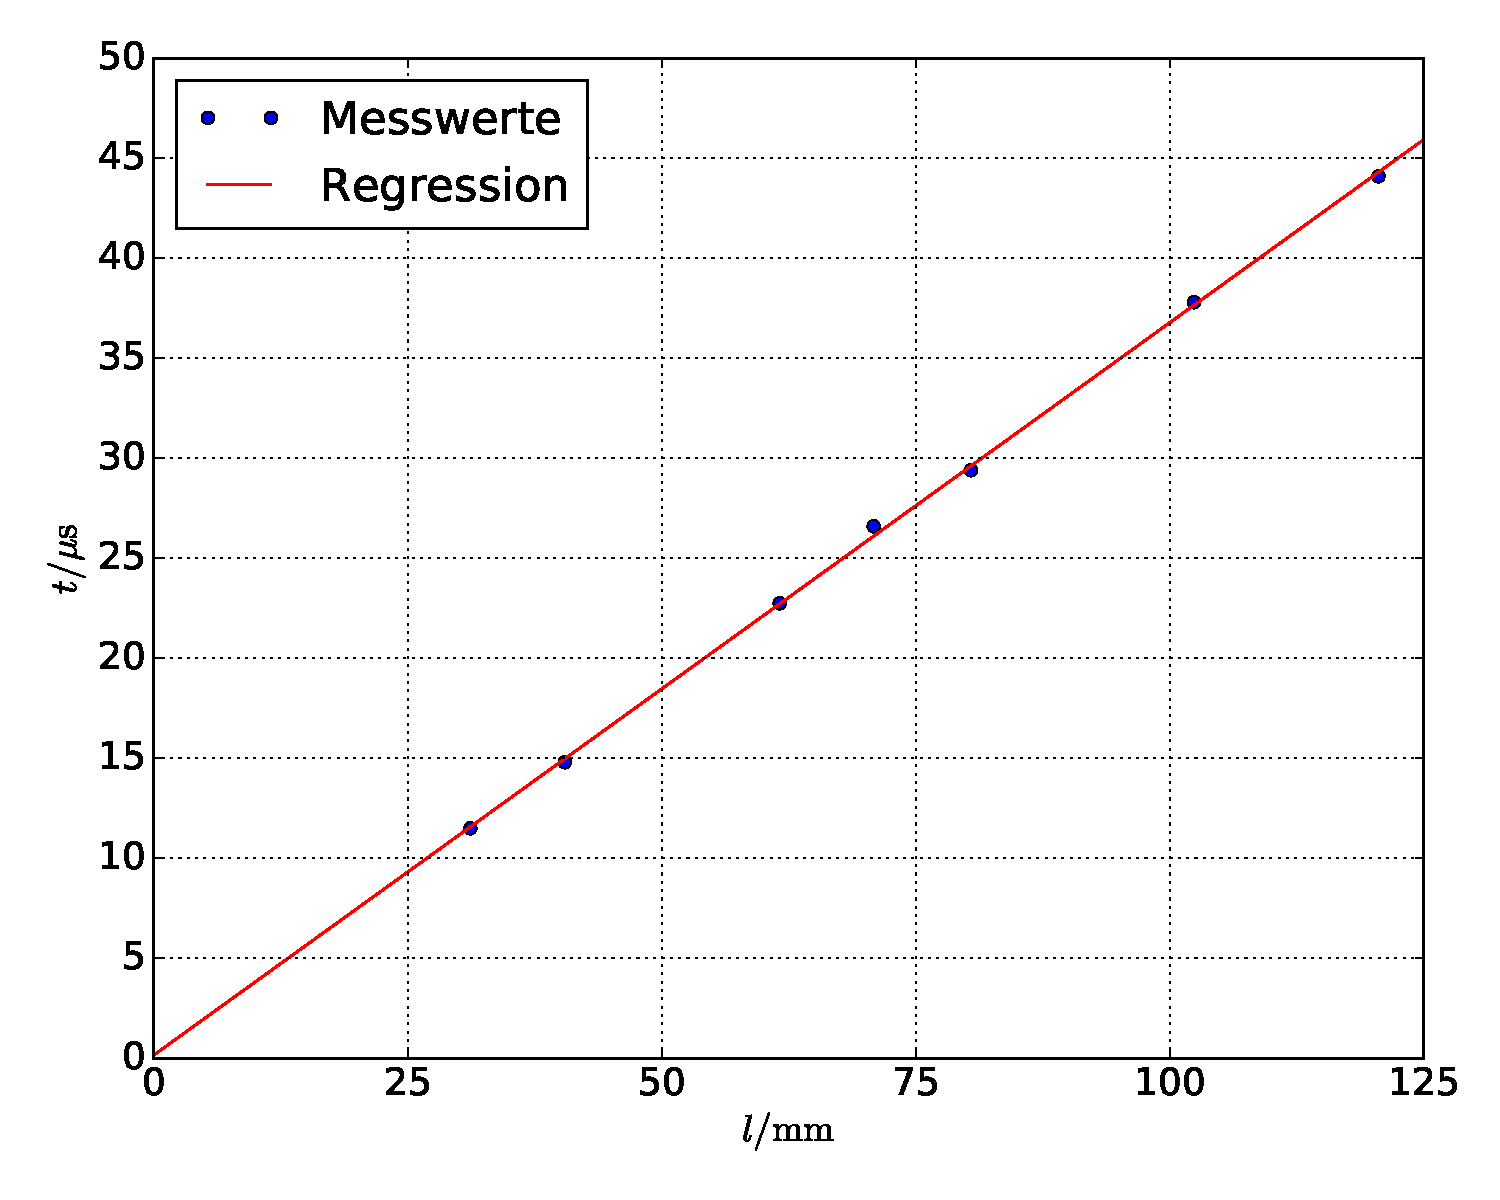
\includegraphics[width=\textwidth]{Imp.pdf}
    \caption{Impuls-Echo-Verfahren}
    \label{abb:1}
  \end{figure}
  \begin{figure}
    \centering
    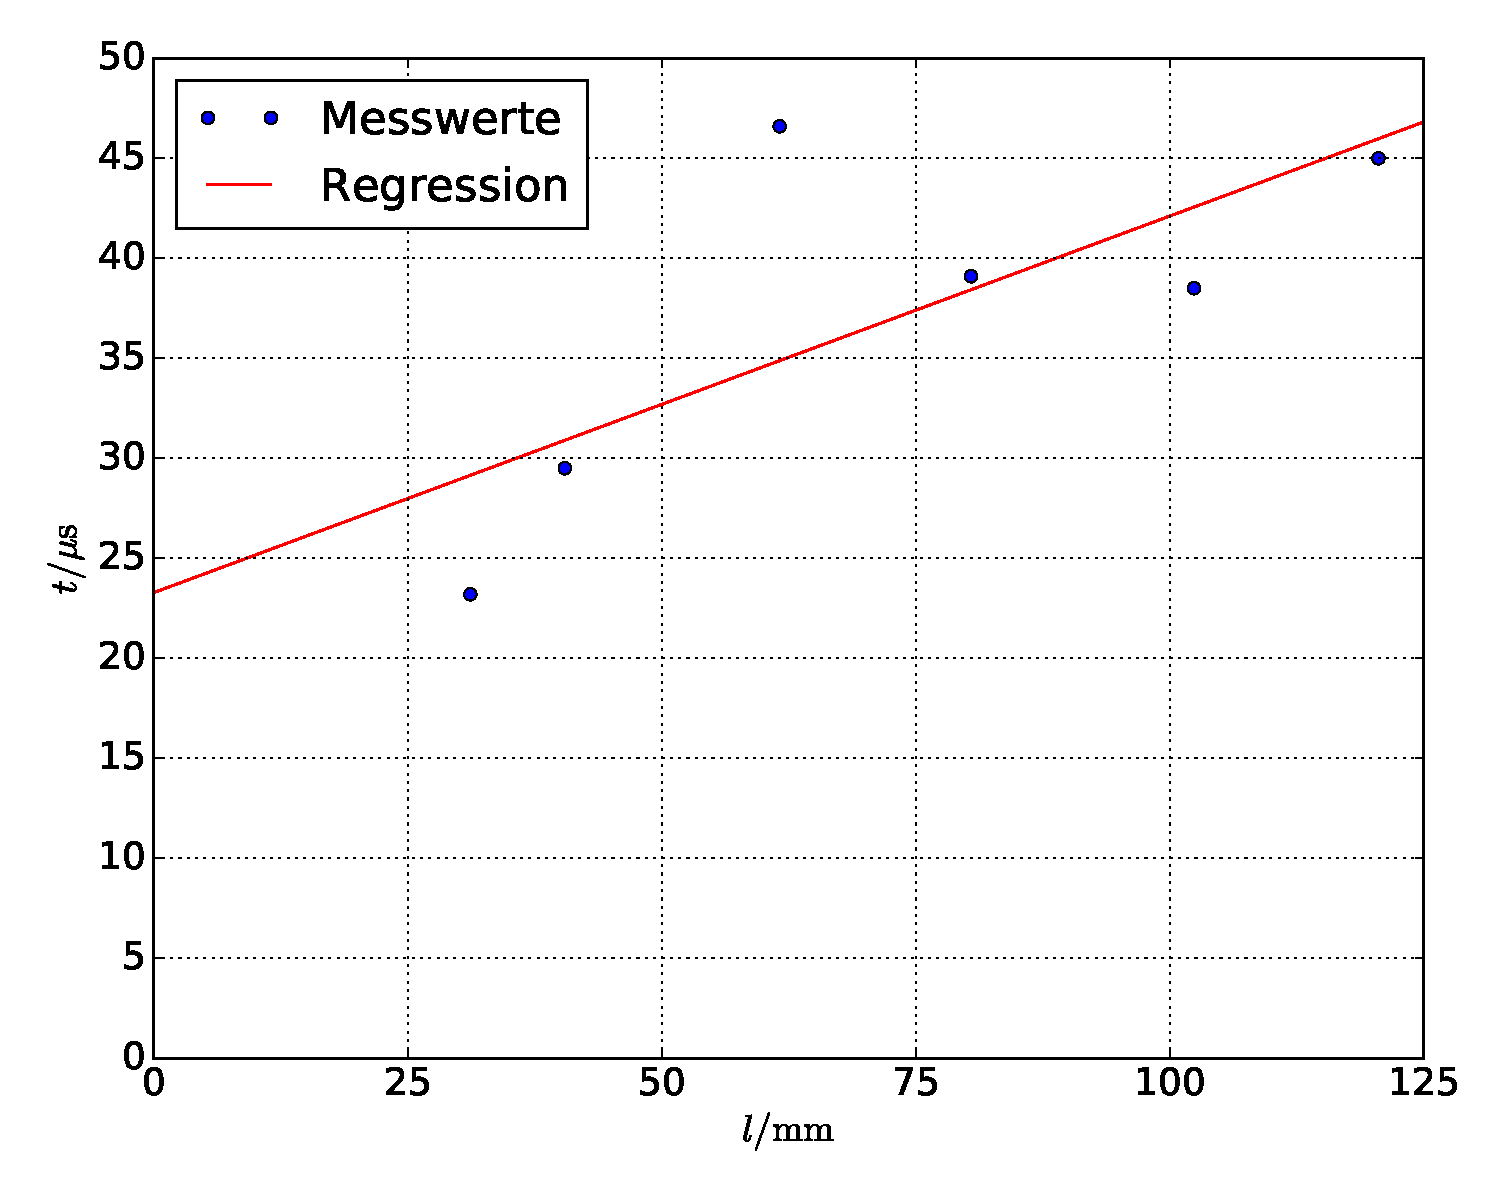
\includegraphics[width=\textwidth]{Dur.pdf}
    \caption{Durchschallverfahren}
    \label{abb:2}
  \end{figure}
\noindent
Dargestellt sind die gemessenen Laufzeiten bei beiden Messmethoden mit Regression.
Insbesondere in \ref{abb:2} erkennt man die Verschiebung des Graphen auf der y-Achse,
verursacht durch die Schalllaufzeit innerhalb der Sonde, deutlich.


\subsection{Betrachtung des Dämpfungsverhaltens von Acryl}
Nun werden die Dämpfungseigenschaften von Acryl betrachtet. Dabei wird die gemessene
Spannungsamplitude des Signals in Abhängigkeit der zurückgelegten Wegstrecke betrachtet.
Zu beachten ist hier: Beim Impuls-Echo-Verfahren wird Verfahrensbedingt die dopplete Strecke zurückgelegt,
manche Amplituden mussten mit Verstärkung gemessen werden. Diese ist in den Tabellen
\ref{tab:1} und \ref{tab:2} als $\textsc{TGC}$-Wert in \si{\decibel} angegeben. Die Umrechnung in einen
linearen Faktor geschieht durch:
  \begin{equation}
    G(g) = 10^{ \left( g \cdot \frac{1}{20} \right)}
    \label{eqqA:1}
  \end{equation}
  mit $\textsc{TGC}$-Wert $g$.
Die Dämpfung verläuft exponentiell, der Dämpfungskoeffizient $\alpha$ wird daher durch Regression
mit einer Funktion:
\begin{equation}
  U(l) = U_0 \cdot e^{\alpha l}
\end{equation}
in $\textsc{phyton-scipy}$ bestimmt. Für das Impuls-Echo-Verfahren ergeben sich:
\begin{align*}
  U_0 &= \SI{0.43(15)}{\volt}\\
  \alpha &= \SI{-19(7)}{\per\metre}
\end{align*}
und für das Durchschallungsverfahren:
\begin{align*}
  U_0 &= \SI{3.1(14)}{\volt}\\
  \alpha &= \SI{-24(6)}{\per\metre}
\end{align*}
Die Verläufe mit Regression sind in den Abbildungen \ref{abb:3} und \ref{abb:4} dargestellt. Dabei sind die gemessenen Signalamplituden in Abhängigkeit
der Signallaufzeit bei beiden Messmethoden mit Regression dargestellt.
\begin{figure}
    \centering
    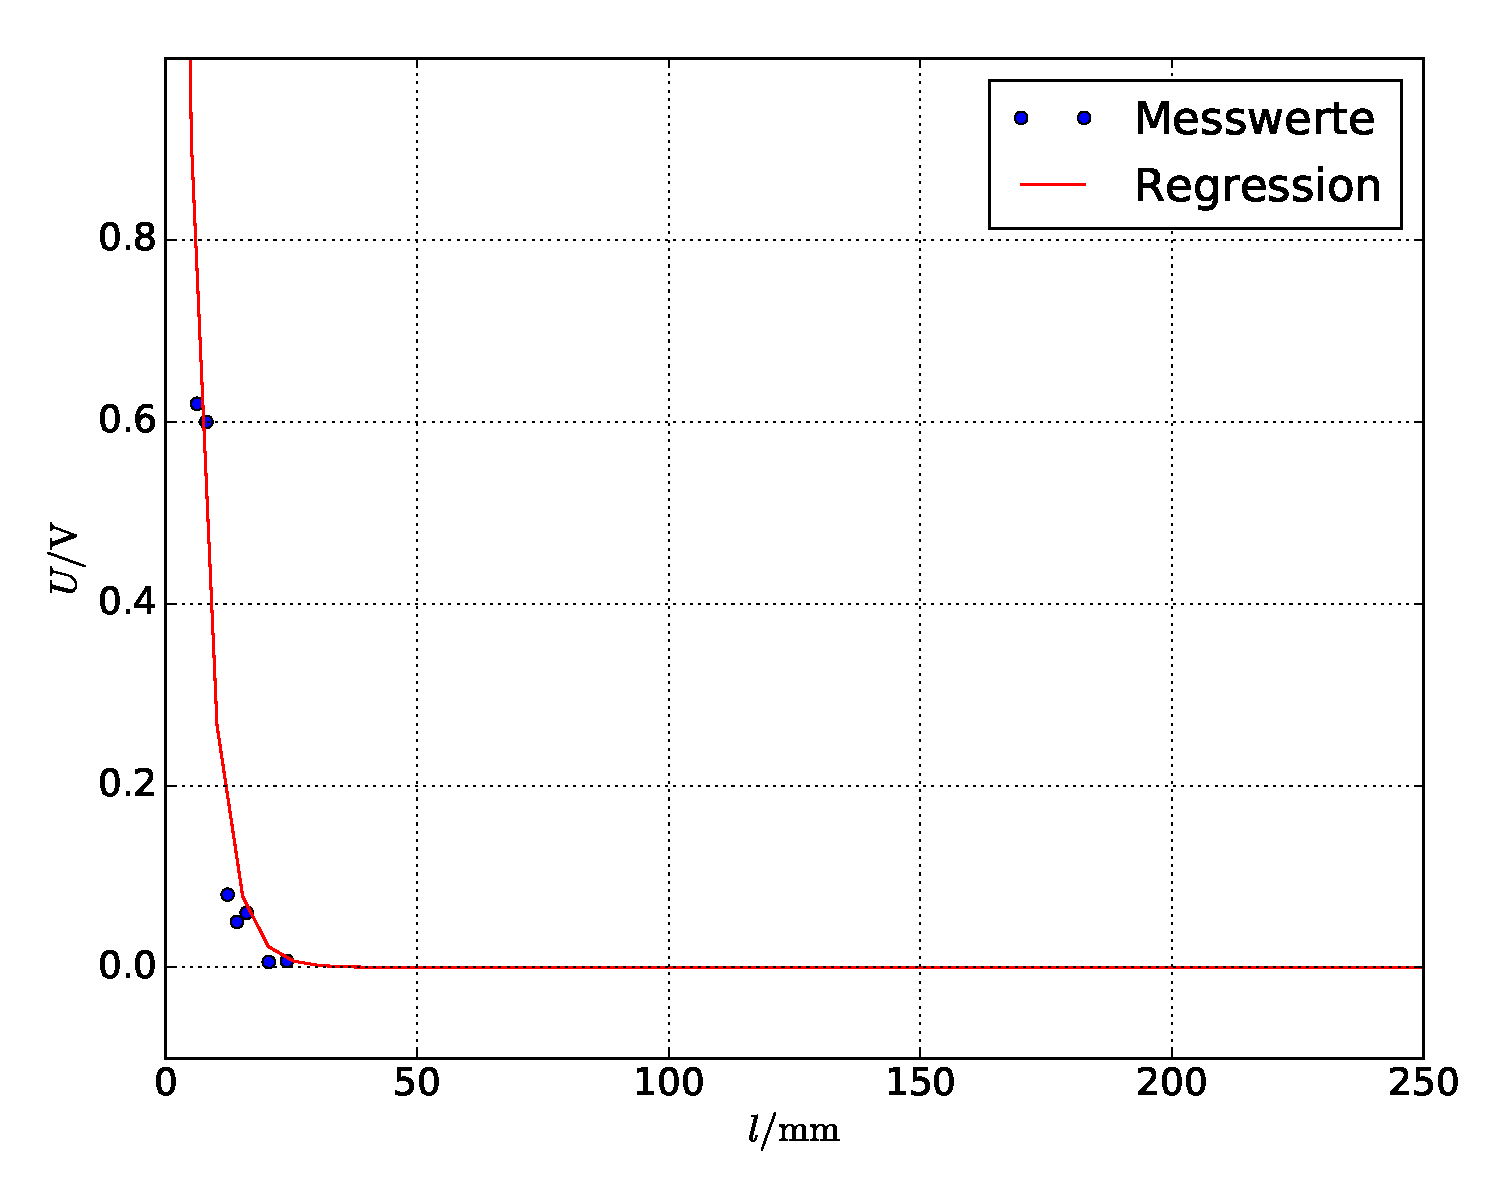
\includegraphics[width=\textwidth]{ImpDump.pdf}
    \caption{Impuls-Echo-Verfahren}
    \label{abb:3}
  \end{figure}
  \begin{figure}
    \centering
    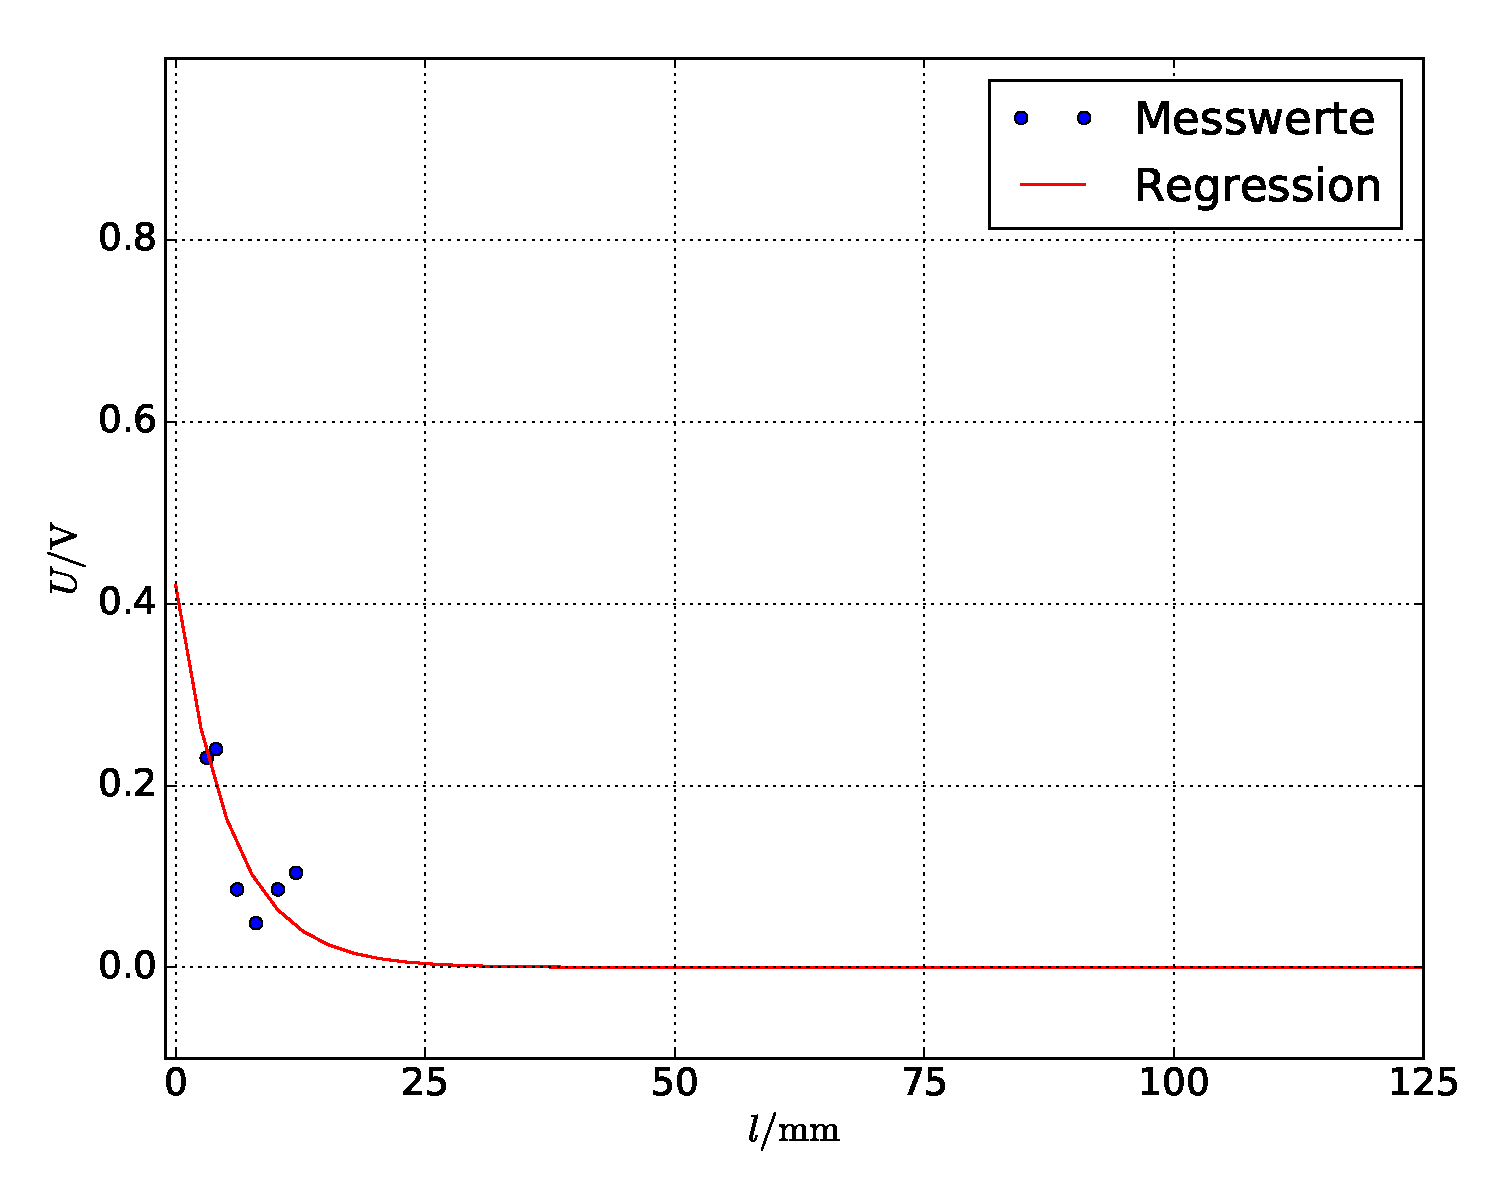
\includegraphics[width=\textwidth]{DurDump.pdf}
    \caption{Durchschallverfahren}
    \label{abb:4}
  \end{figure}
\subsection{Vermessung des Augenmodells}
Die gewonnenen Messwerte sind in Tabelle \ref{tab:3} dargestellt. Für die Schallgeschwindigkeit\cite{anleitung}
in der Glaskörperflüssigkeit gilt $c_{GK} = \SI[per-mode=reciprocal]{1410}{\metre\per\second}$
und für die Linse $c_L = \SI[per-mode=reciprocal]{2500}{\metre\per\second}$. Sind die
Laufzeitdifferenzen $\symup{\Delta}t$ zwischen den Grenzflächen bekannt, kann nach
\begin{equation}
  S = \frac{1}{2} c \cdot \symup{\Delta}t
\end{equation}
der Abstand zwischen den Schichten bestimmt werden. Der Faktor $1/2$ ist notwendig,
da beim Impuls-Echo-Verfahren die doppelten Laufzeiten gemessen werden.
\begin{table}
\centering
  \begin{tabular}{c c}
    \toprule
    Grenzschicht & $\symup{\Delta}t$/\si{\micro\second} \\
    \midrule
    Iris & 5.77 \\
    Linse ein & 8.13 \\
    Linse aus & 9.50 \\
    Retina & 23.60 \\
    \bottomrule
  \end{tabular}
  \caption{Messergebnisse.}
  \label{tab:3}
\end{table}
\begin{table}
  \centering
  \begin{tabular}{c c}
    \toprule
    Grenzschicht & $\frac{l}{3}$/\si{\milli\metre} \\
    \midrule
    Iris & 2.41\\
    Linse ein & 5.38\\
    Linse aus & 5.93\\
    Retina & 12.00\\
    \bottomrule
  \end{tabular}
  \caption{Berechnete Werte.}
  \label{tab:4}
\end{table}
\noindent
Dargestellt sind in \ref{tab:3} die Ergebnisse der Vermessung des Augenmodells im Maßstab 3:1,
angegeben als Verfahrensbedingt doppelte Laufzeiten. In \ref{tab:4} finden sich
die berechneten Abstände zwischen Schallsonde und den angegebenen Grenzschichten
für das Augenmodell (Maßstab 3:1) und zurückgerechnet auf ein menschliches Auge.

\subsection{Bestimmung der Dicke von Acrylplatten mithilfe des Cepstrum}
Das vermessene Cepstrum findet sich in Abbildung \ref{abb:5}. Die daraus erhaltenen
Messwerte finden sich in Tabelle \ref{tab:5}.
\begin{figure}
  \centering
  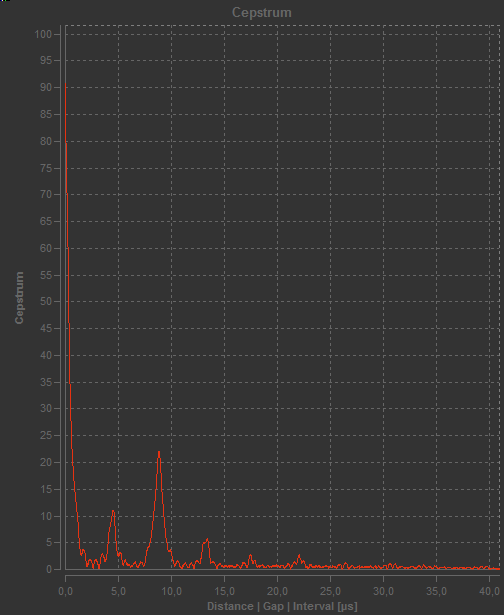
\includegraphics[width=\textwidth]{mehrfachrefl.png}
  \caption{Ausschnitt des aufgenommenen Cepstrums.}
  \label{abb:5}
\end{figure}
\begin{table}
  \centering
  \begin{tabular}{c c }
    \toprule
    Peak & $t$/\si{\micro\second} \\
    \midrule
    1 & 4.5\\
    2 & 8.8\\
    3 & 13.3\\
    4 & 17.4\\
    5 & 22.0\\
    \bottomrule
  \end{tabular}
  \caption{Messwerte.}
  \label{tab:5}
\end{table}
Bei den
Messwerten in \ref{tab:5} gehören 1. und 2. sowie 3. und 4. Messwert so zusammen,
dass 3. und 4. Reflextionen von 1. und 2. sind. Wieder handelt es sich um die doppelten Werte. Messwert 5. ist dann eine "doppelte" Reflexion von 1.
Es ergeben sich also zwei Werte für die Dicke der Platten. Als Schallgeschwindigkeit wird
der aus dem Durchschallverfahren bestimmte Wert genutzt, da sein Fehlerintervall kleiner
ist. In Tabelle \ref{tab:6} sind die bestimmten Werte für die Plattendicke angegeben.
\begin{table}
  \centering
  \begin{tabular}{S S S S S}
    \toprule
    \multicolumn {1}{c}{} & \multicolumn{2}{c}{Platte 1} & \multicolumn {2}{c}{Platte 2}\\
    Paar & {$\symup{\Delta}t$/\si{\micro\second}} & {$d$/\si{\milli\metre}} & {$\symup{\Delta}t$/\si{\micro\second}} & {$d$/\si{\milli\metre}} \\
    \midrule
    1 & 2.372 & \num{6.02(5)} & 4.335 & \num{11.91(9)} \\
    2 & 2.401 & \num{6.08(5)} & 4.380 & \num{11.98(9)} \\
    \bottomrule
  \end{tabular}
  \caption{Berechnete Werte.}
  \label{tab:6}
\end{table}
\begin{table}
  \centering
  \begin{tabular}{c c}
    \toprule
    Platte & $d$/\si{\milli\metre} \\
    \midrule
    1 & 6.01\\
    2 & 11.95\\
    \bottomrule
  \end{tabular}
  \caption{Vergleichswerte.}
  \label{tab:7}
\end{table}
\noindent
Dargestellt sind in \ref{tab:6} die Ergebnisse für beide gemessenen Paare von Peaks.
Die Differenz $\symup{\Delta}t$ der Laufzeiten ist dabei aus den Messwerten (siehe Tabelle \ref{tab:5})
berechnet und halbiert, da die doppelte Laufzeit gemessen wurde. In \ref{tab:7} finden
sich die durch direkte Vermessung der Platten erhaltenen Werte.
\noindent
Die Laufzeitdifferenzen ergeben sich aus
\begin{equation}
  \symup{\Delta}t = \frac{t_2 - t_1}{2}.
\end{equation}
Wieder ist der Faktor $1/2$ notwendig, da doppelte Laufzeiten gemessen wurden. Aus
dem Wert für $\symup{\Delta}t$ lässt sich dann durch $d = ct$ der Durchmesser
der vermessenen Platte bestimmen.
\section{Diskussion}
Bei allen Messwerten ist zu beachten, dass die erhaltenen Abweichungen bei den
hohen Schallgeschwindigkeiten in den Material leicht zu großen Abweichungen führen.
\subsection{Schallgeschwindigkeitsmessung}
Beide Ergebnisse liegen innerhalb der gegenseitigen Messungenauigkeit. Ebenfalls liegt
der Literaturwert\cite{acryl} von \SI{2730}{\metre\per\second} in den Intervallen
beider Ergebnisse. Auffällig ist die große Abweichung zwischen den Werten der sondeninternen
Laufzeit. Da beide Werte aus einer Ausgleichsrechnung mit einem sehr
begrenzten Datensatz gewonnen wurden und keine Literaturwerte vorhanden sind, kann hier nur
vermutet werden. Das Aufnehmen weiterer Messwerte würde helfen, die Ergebnisse zu verifizieren.
\subsection{Dämpfungsverhalten}
Hohe relative Fehler der Werte lassen sich wieder durch den begrenzten Datensatz
erklären. Ebenfalls problematisch sind die langen Laufzeiten bei der Impuls-Echo-Messung.
Die erhaltenen Daten sind daher bereits stärker gedämpft, weshalb die Ausgleichsrechnung
statisch signifikantere Fehler ergeben sollte. Ein Literaturwert\cite{daempf} von \SI{1.41}{\per\centi\metre}
liegt in keinem der beiden Fehlerintervalle. Auch die relativen Fehler sind sehr hoch. Der Schluss eines
systematischen Fehlers liegt nahe.
\subsection{Messung am Augenmodell}
Für das Augenmodell ergeben sich realistische Werte. Der Durchmesser eines Menschlichen
Auges liegt laut Literatur\cite{auge} zwischen \SI{17}{\milli\metre} und \SI{30}{\milli\metre},
je nach Alter des betrachteten Präparates. Der ermittelte Wert trifft daher auf das Auge eines
Jugendlichen zu.
\subsection{Dickenbestimmung per Cepstrum}
Im Vergleich mit den durch direkte Vermessung erhaltenen Werten zeigen sich Abweichungen.
Diese
Abweichungen sind mit \SI{0.07}{\milli\metre} (dies entspricht \SI{0.1}{\percent}) jedoch
vergleichsweise gering.

\newpage
\nocite{*}
\printbibliography
\end{document}
